% Candidate source: src-e83c48821eaac4546df1607aa7bd47f8c49362fe9d091f3ff8accf356722e61c
% Source PDF SHA-256: 0a787b530b939cb104a802de2c27119b5d150bac7c4f0e78b069bc103f381232
% PDF page 1 (printed page 206), question 19.
% Redraw follows visible/hidden edges: square ABCD and rectangle ACEF perpendicular, point M midpoint of EF.
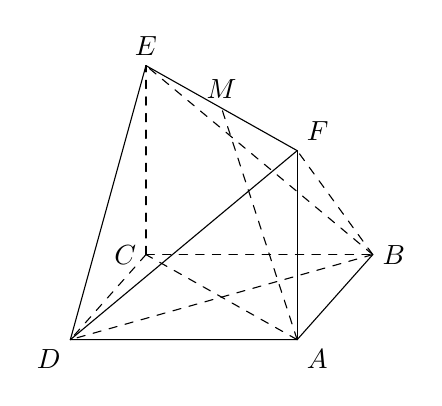
\begin{tikzpicture}[line cap=round,line join=round,>=latex,scale=1.2]
  % Vertex coordinates
  \coordinate (D) at (0,0);
  \coordinate (A) at (2.4,0);
  \coordinate (B) at (3.2,0.9);
  \coordinate (C) at (0.8,0.9);
  \coordinate (F) at (2.4,2.0);
  \coordinate (E) at (0.8,2.9);
  \coordinate (M) at (1.6,2.45);

  % Hidden (dashed) edges
  \draw[dashed] (C) -- (D);
  \draw[dashed] (C) -- (B);
  \draw[dashed] (C) -- (E);
  \draw[dashed] (A) -- (C);
  \draw[dashed] (B) -- (D);
  \draw[dashed] (B) -- (E);
  \draw[dashed] (B) -- (F);
  \draw[dashed] (A) -- (M);

  % Visible (solid) edges
  \draw (D) -- (A) -- (B);
  \draw (A) -- (F);
  \draw (D) -- (E);
  \draw (D) -- (F);
  \draw (E) -- (F);

  % Vertex labels
  \node[below left] at (D) {$D$};
  \node[below right] at (A) {$A$};
  \node[right] at (B) {$B$};
  \node[left] at (C) {$C$};
  \node[above] at (E) {$E$};
  \node[above right] at (F) {$F$};
  \node[above] at (M) {$M$};
\end{tikzpicture}
